\documentclass[10pt, a5paper]{article}
\usepackage{pdfpages}
\usepackage{parallel}
\usepackage[T2A]{fontenc}
\usepackage{ucs}
\usepackage[utf8x]{inputenc}
\usepackage[polish,english,russian]{babel}
\usepackage{hyperref}
\usepackage{rotating}
\usepackage[inner=2cm,top=1.8cm,outer=2cm,bottom=2.3cm,nohead]{geometry}
\usepackage{listings}
\usepackage{graphicx}
\usepackage{wrapfig}
\usepackage{longtable}
\usepackage{indentfirst}
\usepackage{array}
\newcolumntype{P}[1]{>{\raggedright\arraybackslash}p{#1}}
\frenchspacing
\usepackage{fixltx2e} %text sub- and superscripts
\usepackage{icomma} % коскі ў матэматычным рэжыме
\PreloadUnicodePage{4}

\newcommand{\longpage}{\enlargethispage{\baselineskip}}
\newcommand{\shortpage}{\enlargethispage{-\baselineskip}}

\def\switchlang#1{\expandafter\csname switchlang#1\endcsname}
\def\switchlangbe{
\let\saverefname=\refname%
\def\refname{Літаратура}%
\def\figurename{Іл.}%
}
\def\switchlangen{
\let\saverefname=\refname%
\def\refname{References}%
\def\figurename{Fig.}%
}
\def\switchlangru{
\let\saverefname=\refname%
\let\savefigurename=\figurename%
\def\refname{Литература}%
\def\figurename{Рис.}%
}

\hyphenation{admi-ni-stra-tive}
\hyphenation{ex-pe-ri-ence}
\hyphenation{fle-xi-bi-li-ty}
\hyphenation{Py-thon}
\hyphenation{ma-the-ma-ti-cal}
\hyphenation{re-ported}
\hyphenation{imp-le-menta-tions}
\hyphenation{pro-vides}
\hyphenation{en-gi-neering}
\hyphenation{com-pa-ti-bi-li-ty}
\hyphenation{im-pos-sible}
\hyphenation{desk-top}
\hyphenation{elec-tro-nic}
\hyphenation{com-pa-ny}
\hyphenation{de-ve-lop-ment}
\hyphenation{de-ve-loping}
\hyphenation{de-ve-lop}
\hyphenation{da-ta-ba-se}
\hyphenation{plat-forms}
\hyphenation{or-ga-ni-za-tion}
\hyphenation{pro-gramming}
\hyphenation{in-stru-ments}
\hyphenation{Li-nux}
\hyphenation{sour-ce}
\hyphenation{en-vi-ron-ment}
\hyphenation{Te-le-pathy}
\hyphenation{Li-nux-ov-ka}
\hyphenation{Open-BSD}
\hyphenation{Free-BSD}
\hyphenation{men-ti-on-ed}
\hyphenation{app-li-ca-tion}

\def\progref!#1!{\texttt{#1}}
\renewcommand{\arraystretch}{2} %Іначай формулы ў матрыцы зліпаюцца з лініямі
\usepackage{array}

\def\interview #1 (#2), #3, #4, #5\par{

\section[#1, #3, #4]{#1 -- #3, #4}
\def\qname{LVEE}
\def\aname{#1}
\def\q ##1\par{{\noindent \bf \qname: ##1 }\par}
\def\a{{\noindent \bf \aname: } \def\qname{L}\def\aname{#2}}
}

\def\interview* #1 (#2), #3, #4, #5\par{

\section*{#1\\{\small\rm #3, #4. #5}}

\def\qname{LVEE}
\def\aname{#1}
\def\q ##1\par{{\noindent \bf \qname: ##1 }\par}
\def\a{{\noindent \bf \aname: } \def\qname{L}\def\aname{#2}}
}

\begin{document}
\title{Использование архитектуры  EAV в Opensource-проектах\footnote{\url{vitalyok@tut.by}, \url{http://lvee.org/ru/abstracts/172}}}
\author{Виталий Сороко, Гродно, belarus}
\maketitle
\begin{abstract}
Entity–attribute–value model (EAV) is a very flexible data model used in various open source projects. This data model has many advantages and disadvantages so it is not suitable for wide application. But sometimes it is highly recommended to use EAV in design and development process.

Cases are decribed, in which it is preferable to use EAV data model. EAV is completely compared with the standard relational data model and  some examples of  successfully integration EAV in ready-to-use open source solutions are given.
\end{abstract}

Entity–attribute–value model (EAV) – это модель данных, которая благодаря использованию сущностей, атрибутов и их значений обеспечивает большую гибкость при создании новых данных. Это означает, что при создании нового типа товара в интернет магазине нет никакой необходимости создавать новые таблицы и поля в базе данных. Более того благодаря использованию этой модели данных можно с лёгкостью создать один товар из нескольких уже существующих (например «подарочный набор»). Тем не менее использование модели  EAV не ограничивается только интернет магазинами: некоммерческая организация Apache Software Foundation использует её в проекте Apache UIMA, а некоторые системы баз данных, такие как InfinityDB, изначально имеют поддержку модели данных EAV.

\begin{figure}[h!]
  \centering
  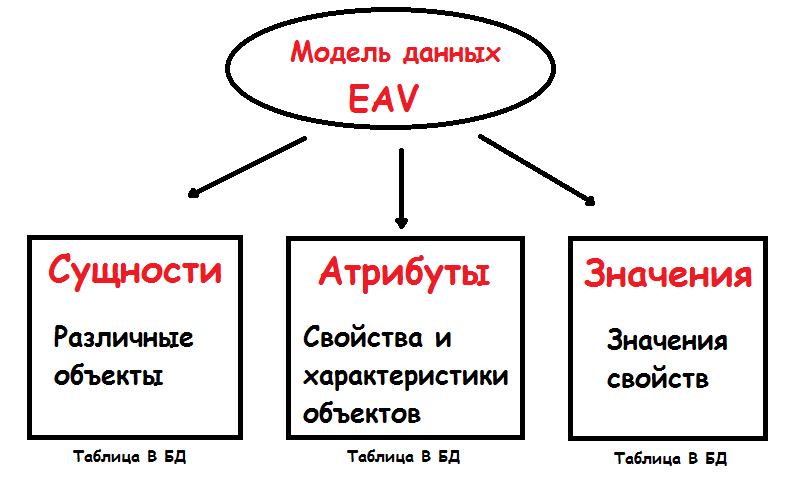
\includegraphics[width=10cm]{w_10_2016_Soroko1.png}
  \caption {Общая схема EAV в виде трёх таблиц}\label{Soroko1}
\end{figure} 

Тем не менее у модели данных EAV, как и у всех других моделей данных, есть свои преимущества и недостатки и это в некоторых случаях ограничивает возможность использования данной модели.

Главными плюсами модели данных EAV являются:

\begin{enumerate}
\item Гибкая и универсальная структура данных (можно менять количество свойств без изменения полей в таблицах);
\item Относительная простота при добавлении или изменении характеристики товара;
\item При правильной реализации избыточность данных почти отсутствует.
\end{enumerate}

Основные минусы EAV:
\begin{enumerate}
\item Для вставки данных обычно используется несколько запросов;
\item Не очень быстрая выборка данных в случае реализации с большим количеством таблиц и высокая нагрузка на сервер при больших объемах данных в связи с невозможностью применения стандартных способов индексации;
\item Иногда возникают трудности в обеспечении целостности данных.
\end{enumerate}

\begin{figure}[h!]
  \centering
  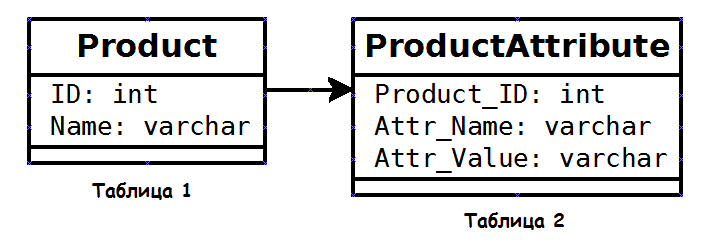
\includegraphics[width=10cm]{w_10_2016_Soroko2.png}
  \caption {Простейшая реализация EAV в виде двух таблиц}\label{Soroko2}
\end{figure} 

В настоящее время модель данных EAV используется в таких Opensource проектах как  Magento Community Edition, EAV-Django и др.  Необходимо отметить, что модель данных EAV не получила очень широкого распространения не только из-за своих технических минусов, но также в результате её неполного понимания со стороны разработчиков. Как правило только те, кто разобрался с принципом работы этой модели и попробовал её в реальной среде, могут объективно судить о её преимуществах и недостатках,  а также рекомендовать её к использованию в той или иной ситуации и именно поэтому, очень важно полностью понять основные принципы  организации её работы. В упрощённом виде реализация модели EAV может быть в виде двух или трех таблиц (см. рис.~\ref{Soroko1} и рис.~\ref{Soroko2}).

Однако в реальных проектах реализация обычно сложнее, и на то есть определенные причины, такие как оптимизация скорости обработки запросов и уменьшение общего количества записей в таблицах.Так, например, в Magento CMS CE для реализации данной модели используется больше десятка таблиц. Как вы могли узнать из описание недостатков выше, иногда гибкость может трансформироваться в падение производительности всей системы. Тем не менее, в настоящее время уже разработаны различные способы решения этой проблемы. Итого, главная рекомендация по применению следующая: EAV рекомендуется использовать только исходя из плюсов, а именно в случаях если характеристики для товаров очень динамичны и часто изменяются и вы не ограничены в серверных ресурсах.

\end{document}
